% ------------------------------------------------------------------------------
% TYPO3 CMS 7.1 - What's New - Chapter "Backend User Interface" (Russian Version)
%
% @author		Michael Schams <schams.net>
% @translation	Andrey Aksenov <aksenovaa@bk.ru>
% @license		Creative Commons BY-NC-SA 3.0
% @link			http://typo3.org/download/release-notes/whats-new/
% @language		Russian
% ------------------------------------------------------------------------------
% LTXE-CHAPTER-UID:		e7264f0e-3f82290d-94c50cda-fb2d8e66
% LTXE-CHAPTER-NAME:	Backend User Interface
% ------------------------------------------------------------------------------

\section{BackendUI}
\begin{frame}[fragile]
	\frametitle{Backend / Внутренний интерфейс}

	\begin{center}\huge{Глава 1:}\end{center}
	\begin{center}\huge{\color{typo3darkgrey}\textbf{Backend / Внутренний интерфейс}}\end{center}

\end{frame}

% ------------------------------------------------------------------------------
% LTXE-SLIDE-START
% LTXE-SLIDE-UID:		f8e37b64-85916b07-1d7c6bbd-49fe4fa3
% LTXE-SLIDE-ORIGIN:	d5fddde9-b3ee31c0-f0509300-40a2928e English
% LTXE-SLIDE-TITLE:		Date/Time Picker
% LTXE-SLIDE-REFERENCE:	Breaking-62925-RemoveExtJsDateTimePicker.rst
% ------------------------------------------------------------------------------

\begin{frame}[fragile]
	\frametitle{Backend / Внутренний интерфейс}
	\framesubtitle{Вид и ощущение: выбор даты/времени}

	Элемент выбора даты/времени был заменён альтернативой из Bootstrap
	\begin{figure}
		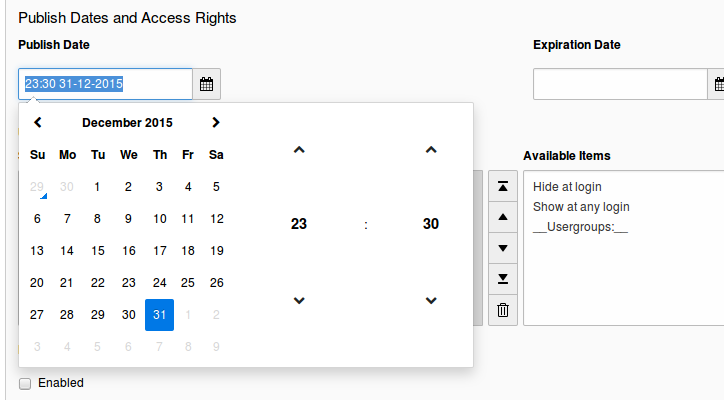
\includegraphics[width=0.75\linewidth]{BackendUserInterface/be-datepicker.png}
	\end{figure}

\end{frame}

% ------------------------------------------------------------------------------
% LTXE-SLIDE-START
% LTXE-SLIDE-UID:		ca2676c3-98162e7a-3cdaa08a-e2663427
% LTXE-SLIDE-ORIGIN:	1c391eec-dfb1dfa6-f783ae7a-d0b214ae English
% LTXE-SLIDE-TITLE:		Functions Module
% LTXE-SLIDE-REFERENCE:	Breaking-63310-Wizard-Modules-Moved.rst
% ------------------------------------------------------------------------------

\begin{frame}[fragile]
	\frametitle{Backend / Внутренний интерфейс}
	\framesubtitle{Вид и ощущение: модуль Функции}

	"Создать страницы/Create Pages" и "Упорядочить страницы/Sort Pages" перемещено в: \texttt{Веб => Функции}\newline
	\smaller (в TYPO3 CMS < 7.1, они находились в "\texttt{Веб => Функции => Мастера}")

	\begin{figure}
		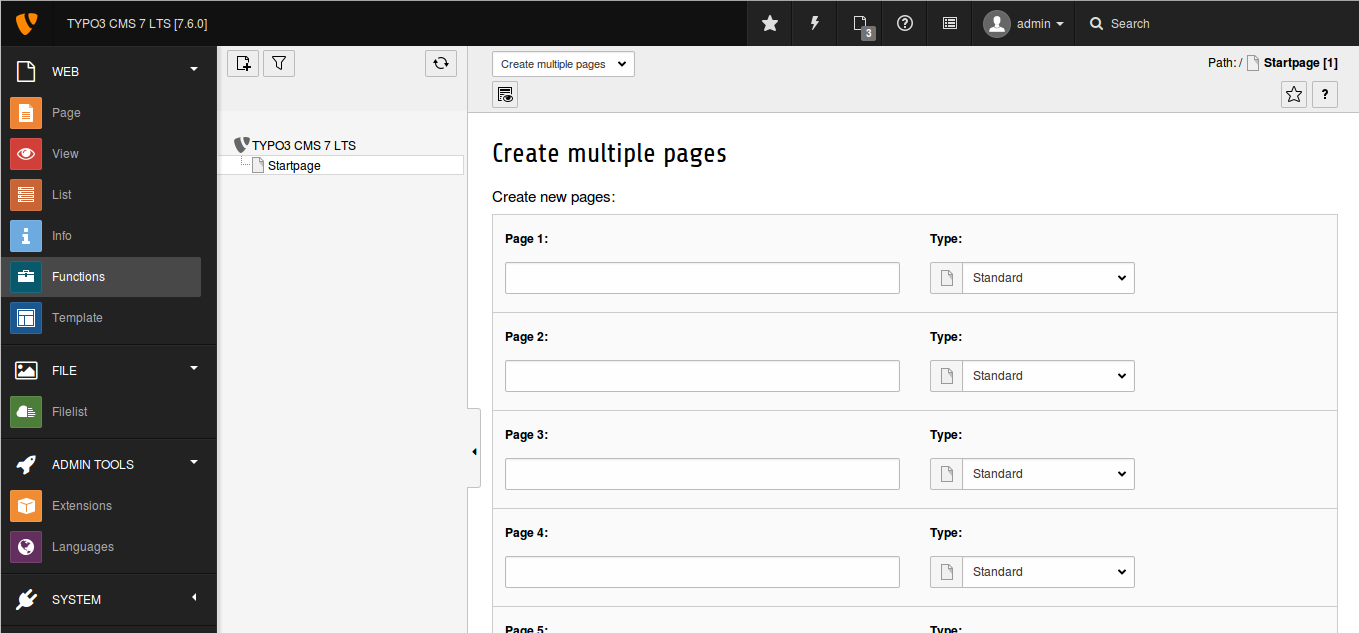
\includegraphics[width=0.80\linewidth]{BackendUserInterface/be-functions.png}
	\end{figure}


\end{frame}

% ------------------------------------------------------------------------------
% LTXE-SLIDE-START
% LTXE-SLIDE-UID:		55be3a05-de40f335-52be7af6-01a41ad0
% LTXE-SLIDE-ORIGIN:	dd127630-5ccc729a-835e5836-e8796962 English
% LTXE-SLIDE-TITLE:		Access Module: Leave Unchaged
% LTXE-SLIDE-REFERENCE:	Feature-15619-LeaveUnchagedInAccessModule.rst
% ------------------------------------------------------------------------------

\begin{frame}[fragile]
	\frametitle{Backend / Внутренний интерфейс}
	\framesubtitle{Вид и ощущение: модуль Доступ}

	Module \texttt{Веб => Доступ} позволяет оставить тех же пользователя/группу\newline
	при переназначении прав

	\begin{figure}
		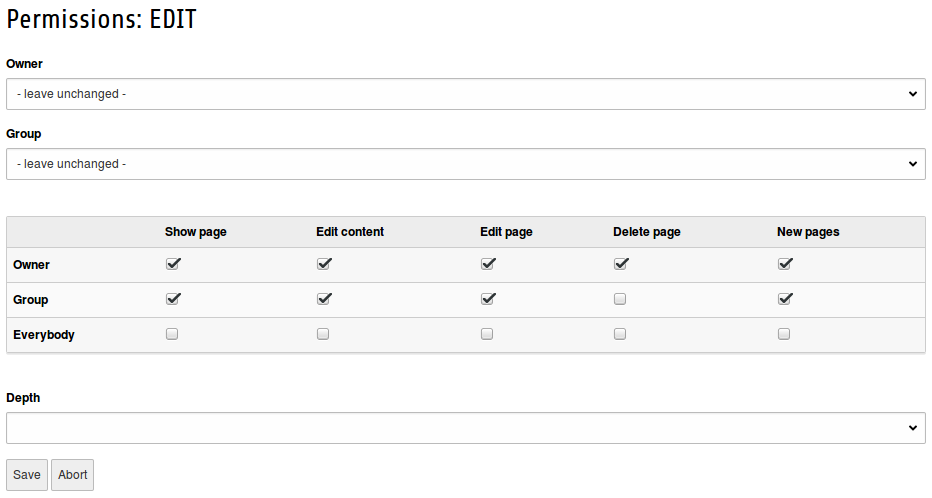
\includegraphics[width=0.75\linewidth]{BackendUserInterface/be-access.png}
	\end{figure}

\end{frame}

% ------------------------------------------------------------------------------
% LTXE-SLIDE-START
% LTXE-SLIDE-UID:		6d1e9c13-e0e4c347-4b77430c-c58cfaf2
% LTXE-SLIDE-ORIGIN:	eb6cc867-e4f5d0d3-ea06672c-7ccdf227 English
% LTXE-SLIDE-TITLE:		Icons in List Module
% LTXE-SLIDE-REFERENCE:	Feature-63207-SplitActionButtonsIntoGroups.rst
% ------------------------------------------------------------------------------

\begin{frame}[fragile]
	\frametitle{Backend / Внутренний интерфейс}
	\framesubtitle{Вид и ощущение: значки в модуле Список}

	Значки ("кнопки действий") в модуле Список разбиты на две группы\newline
	\smaller (сначала основные действия (читать, обновить, удалить), затем - второстепенные)

	\begin{figure}
		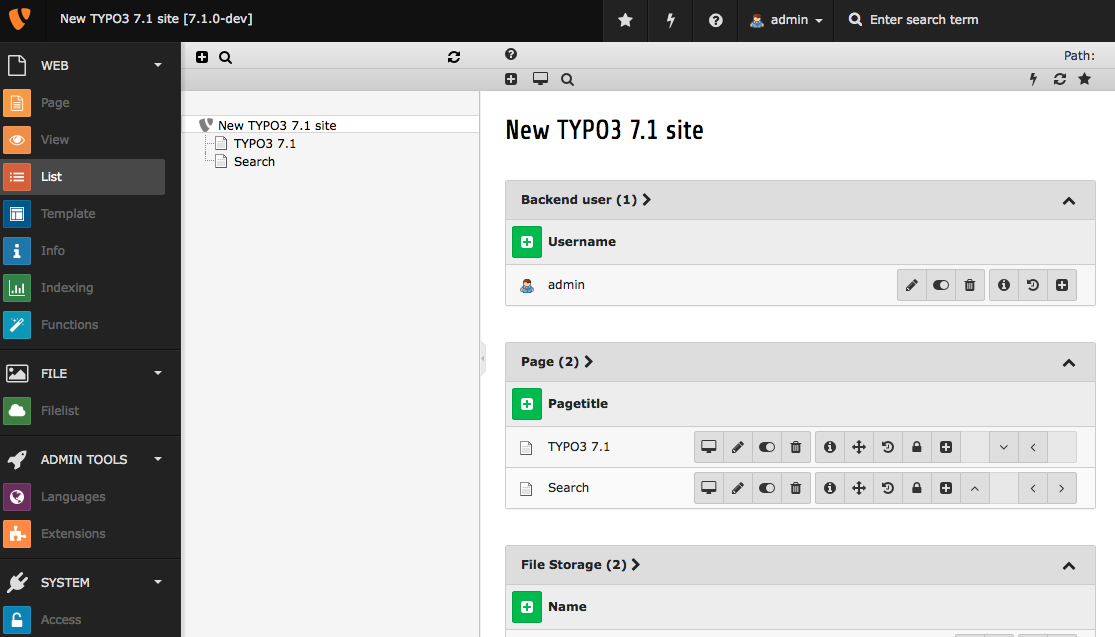
\includegraphics[width=0.75\linewidth]{BackendUserInterface/be-icons.png}
	\end{figure}

\end{frame}

% ------------------------------------------------------------------------------
